\section{Introduction}

\begin{frame}{Introduction}
  \framesubtitle{Why Vision Transformers ?}
  \begin{itemize}
    \item Vision Transformers (ViTs) have revolutionized image recognition.
    \item Traditional ViTs require large datasets and heavy computation.
    \item TinyViT is a simplified alternative, retaining core transformer components while being computationally efficient.
  \end{itemize}
\end{frame}

\begin{frame}{Vision Transformer Architecture}
  \framesubtitle{Take a look at the Architecture}
  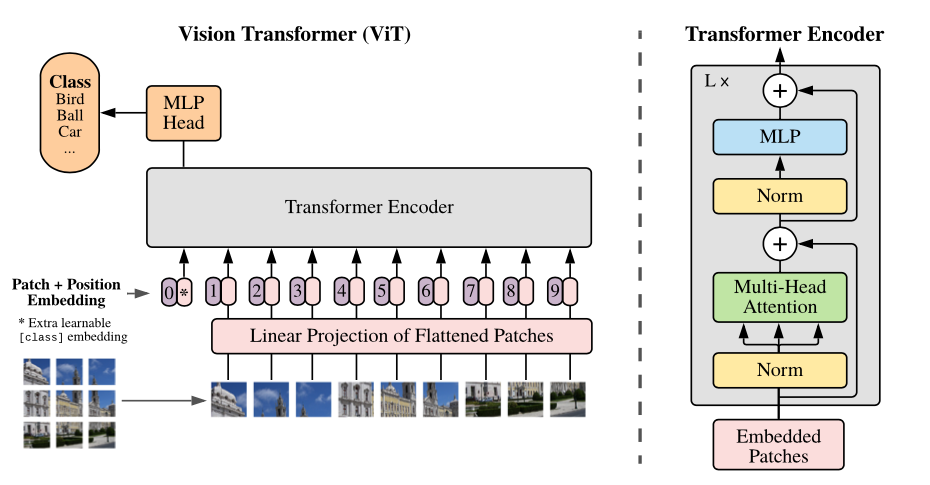
\includegraphics[width=\textwidth]{images/vit-architecture.png}
\end{frame}

\begin{frame}{Vision Transformer Overview}
  \framesubtitle{Follow the steps}
  \begin{itemize}
    \item Inspired by NLP transformers (Vaswani et al., 2017).
    \item Treats images as sequences of patches instead of processing pixels directly.
    \item Uses a stack of transformer encoder blocks for feature extraction.
  \end{itemize}
  \begin{columns}
    \begin{column}{0.2\textwidth}
      \begin{block}{Step 1}
        Patch \\ Embedding
      \end{block}
    \end{column}
    \begin{column}{0.2\textwidth}
      \begin{block}{Step 2}
        Positional Encoding
      \end{block}
    \end{column}
    \begin{column}{0.2\textwidth}
      \begin{block}{Step 3}
        Transformer Encoder
      \end{block}
    \end{column}
    \begin{column}{0.2\textwidth}
      \begin{block}{Step 4}
        Classification Head
      \end{block}
    \end{column}
  \end{columns}
\end{frame}